\documentclass[12pt]{article}

\input preamble

\title{Principles of Parallel Architecture\\
Project Report 1}
\author{Xitong Liu \\
xliu@ece.udel.edu}

\begin{document}

\maketitle

\section{Project Description}
The class project is designed to explore and understand 
a particular aspect of parallel architecture and parallel 
computing.

I choose Matrix Multiply as the topic of my project and 
use OpenMP to implement parallel computation.

\section{Implementation}
The intuitive way to implement matrix multiplication in a 
parallel is to divide the matrix evenly into several
sub-parts, 

\begin{figure}[h!]
	\begin{center}
		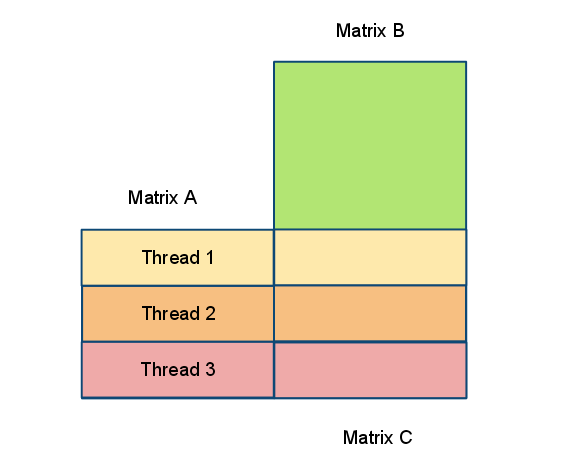
\includegraphics[width=0.7\textwidth, angle=0]{matrix-divide.png}
		\caption{\label{fig:matrix-divide}Divide the matrix evenly by the number of threads}
	\end{center}
\end{figure}

\end{document}

\begin{comment}
\begin{figure}[h!]
	\begin{center}
		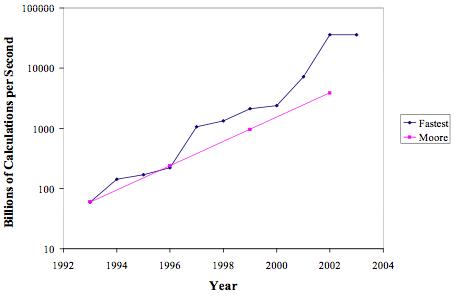
\includegraphics[width=0.7\textwidth, angle=0]{fatest.png}
		\caption{\label{fig:fatest}Fatest SuperComputer in the world}
	\end{center}
\end{figure}
\end{comment}